% ==========================================================
% ENTREGA 1 — A pergunta do trabalho
% Versão compatível: article + natbib (sem abntex2)
%
% Compilar:
%   RStudio: botão "Compile PDF" (com knitr configurado)
%   Terminal: Rscript -e "knitr::knit2pdf('entrega-1-pergunta.Rnw')"
% ==========================================================
\documentclass[12pt,a4paper,oneside]{article}\usepackage[]{graphicx}\usepackage[]{xcolor}
% maxwidth is the original width if it is less than linewidth
% otherwise use linewidth (to make sure the graphics do not exceed the margin)
\makeatletter
\def\maxwidth{ %
  \ifdim\Gin@nat@width>\linewidth
    \linewidth
  \else
    \Gin@nat@width
  \fi
}
\makeatother

\definecolor{fgcolor}{rgb}{0.345, 0.345, 0.345}
\newcommand{\hlnum}[1]{\textcolor[rgb]{0.686,0.059,0.569}{#1}}%
\newcommand{\hlsng}[1]{\textcolor[rgb]{0.192,0.494,0.8}{#1}}%
\newcommand{\hlcom}[1]{\textcolor[rgb]{0.678,0.584,0.686}{\textit{#1}}}%
\newcommand{\hlopt}[1]{\textcolor[rgb]{0,0,0}{#1}}%
\newcommand{\hldef}[1]{\textcolor[rgb]{0.345,0.345,0.345}{#1}}%
\newcommand{\hlkwa}[1]{\textcolor[rgb]{0.161,0.373,0.58}{\textbf{#1}}}%
\newcommand{\hlkwb}[1]{\textcolor[rgb]{0.69,0.353,0.396}{#1}}%
\newcommand{\hlkwc}[1]{\textcolor[rgb]{0.333,0.667,0.333}{#1}}%
\newcommand{\hlkwd}[1]{\textcolor[rgb]{0.737,0.353,0.396}{\textbf{#1}}}%
\let\hlipl\hlkwb

\usepackage{framed}
\makeatletter
\newenvironment{kframe}{%
 \def\at@end@of@kframe{}%
 \ifinner\ifhmode%
  \def\at@end@of@kframe{\end{minipage}}%
  \begin{minipage}{\columnwidth}%
 \fi\fi%
 \def\FrameCommand##1{\hskip\@totalleftmargin \hskip-\fboxsep
 \colorbox{shadecolor}{##1}\hskip-\fboxsep
     % There is no \\@totalrightmargin, so:
     \hskip-\linewidth \hskip-\@totalleftmargin \hskip\columnwidth}%
 \MakeFramed {\advance\hsize-\width
   \@totalleftmargin\z@ \linewidth\hsize
   \@setminipage}}%
 {\par\unskip\endMakeFramed%
 \at@end@of@kframe}
\makeatother

\definecolor{shadecolor}{rgb}{.97, .97, .97}
\definecolor{messagecolor}{rgb}{0, 0, 0}
\definecolor{warningcolor}{rgb}{1, 0, 1}
\definecolor{errorcolor}{rgb}{1, 0, 0}
\newenvironment{knitrout}{}{} % an empty environment to be redefined in TeX

\usepackage{amsmath}
\usepackage{alltt}

% --- Codificação e idioma ---
\usepackage[T1]{fontenc}
\usepackage{lmodern}
\usepackage[brazilian,english]{babel}

% --- Matemática e tabelas ---
\usepackage{amsmath,amssymb}
\usepackage{icomma}
\usepackage{booktabs}
\usepackage{array}

% --- Layout ---
\usepackage[margin=2.5cm]{geometry}
\usepackage{setspace}

% --- Figuras ---
\usepackage{graphicx}

% --- Hyperlinks ---
\usepackage[hidelinks]{hyperref}

% --- Citações (universal: natbib) ---
\usepackage[round,authoryear]{natbib}
\bibliographystyle{plainnat}

% --- Compatibilidade com os comandos do abntex2 usados no texto ---
\providecommand{\citeonline}[1]{\citet{#1}}
\providecommand{\fonte}[1]{\par\medskip\noindent{\footnotesize Fonte: #1}}
\providecommand{\textual}{}
\providecommand{\postextual}{}

% ----------------------------------------------------------
% DADOS DA ENTREGA
% ----------------------------------------------------------
\title{A pergunta do trabalho: \textit{Quanto a mortalidade de 60 a 69 anos
na Baixada Santista depende de onde (município) e de quando (ano)?}}
\author{Ivan, Gustavo e Jorge}
\date{\today}

\newcommand{\nomecurso}{Tecnologia em Ciência de Dados}
\newcommand{\nomedisciplina}{Teoria do Aprendizado Estatístico}
\newcommand{\nomeprofessor}{Prof.\ Dr.\ João Paulo Ferreira de Mello}
\newcommand{\repositorio}{proj\_ivan\_gustavo\_jorge\_IPDM}
\newcommand{\integrantes}{%
  Ivan -- RA 1999000 \\
  Gustavo -- RA 2004000 \\
  Jorge -- RA 2006000%
}
\IfFileExists{upquote.sty}{\usepackage{upquote}}{}
\begin{document}





\selectlanguage{brazilian}
\frenchspacing

\maketitle

\begin{center}
  \small
  Fatec Baixada Santista -- Rubens Lara \\
  \nomecurso{} \quad|\quad \nomedisciplina{} \quad|\quad \nomeprofessor{} \\[0.4em]
  \integrantes \\[0.4em]
  Repositório: \texttt{\repositorio}
\end{center}

\textual

% ==========================================================================
\section{Introdução}
% ==========================================================================
O monitoramento da mortalidade é essencial para o planejamento de políticas públicas de saúde, sobretudo para a população idosa (60 a 69 anos), que demanda maior atenção e recursos do sistema de saúde. Compreender como essa mortalidade varia na Baixada Santista pode ajudar na alocação mais eficiente de recursos e na identificação de municípios que necessitam de intervenções prioritárias. O presente texto apresenta o banco de dados escolhido, formula a pergunta do trabalho e mostra que os dados têm condição de respondê-la, auxiliando as secretarias de saúde da região.

Referências entram pela NBR 10520. Com o autor ao fim da frase, o formato sai
entre parênteses \cite{james2021}; com o autor no corpo do texto, use
\verb|\citeonline| --- segundo \citeonline{bruce2019}, a escolha da métrica vem
antes da escolha do modelo.

% ==========================================================================
\section{O banco de dados e o problema}
% ==========================================================================
O banco de dados utilizado é o Índice Paulista de Desempenho Municipal (IPDM) da Baixada Santista, mantido pela Fundação Seade \cite{fonte_dados}. Cada linha representa o registro de um município da Baixada Santista em um determinado ano. As colunas principais incluem indicadores sociais (como riqueza e escolaridade) e a taxa de mortalidade na faixa de 60 a 69 anos. O conjunto usado tem $n = \text{54}$ observações e $p = \text{13}$ preditores candidatos.

A escolha deste banco se justifica pela relevância e disponibilidade de dados consistentes sobre as condições de vida e saúde na região. O \emph{problema} a ser resolvido envolve a decisão, por parte das secretarias de saúde da Baixada Santista, de onde priorizar a atenção e os recursos voltados à população de 60 a 69 anos. Uma resposta baseada em dados permitiria que a gestão regional sinalizasse e priorizasse áreas de maior risco com mais segurança do que a abordagem atual.

% ==========================================================================
\section{A pergunta}
% ==========================================================================
A pergunta central do trabalho é: \textit{Quanto a mortalidade de 60 a 69 anos varia com onde (município) e quando (ano) — e quais municípios ficam acima do esperado para o seu ano?} A Tabela~\ref{tab:ficha} detalha os sete campos que a definem.

\begin{table}[htb]
  \centering
  \caption{Ficha da pergunta}
  \label{tab:ficha}
  \small
  \begin{tabular}{@{}p{0.30\textwidth}p{0.62\textwidth}@{}}
    \toprule
    \textbf{Campo} & \textbf{Preenchimento} \\
    \midrule
    1. A pergunta, em uma frase & \textit{Quanto a mortalidade de 60 a 69 anos varia com onde (município) e quando (ano) — e quais municípios ficam acima do esperado para o seu ano?} \\
    2. Resposta $Y$: coluna, tipo, unidade & \texttt{mortalidade\_60\_69} ---
       quantitativa --- \textit{mortes por mil hab.} \\
    3. Preditores $X$: quais e quantos & \textit{\texttt{municipio} (9 níveis) e \texttt{ano} como categoria (6 níveis)} \quad ($p = \text{13}$) \\
    4. Tipo: as três decisões & supervisionado; regress\~ao;
       \textit{inferência} \\
    5. Métrica & RMSE, na unidade de $Y$ em validação cruzada (5 dobras) \\
    6. Linha de base a bater & RMSE = 3,85 \quad (chutar sempre a m\'edia) \\
    7. Dono do problema & \textit{Secretarias de saúde da Baixada: decidir onde priorizar a atenção à população de 60 a 69 anos} \\
    \bottomrule
  \end{tabular}
  \fonte{Elaborada pelos autores.}
\end{table}

A abordagem escolhida é de inferência, pois o objetivo principal é entender e explicar o comportamento da variável de resposta com base nos preditores, identificando desvios e padrões estruturais. Conforme evidenciado no campo 7, a resposta pode influenciar diretamente a tomada de decisão das secretarias de saúde da Baixada Santista na priorização de recursos.

% ==========================================================================
\section{Defesa da pergunta}
% ==========================================================================
A Tabela~\ref{tab:diag} reúne as quatro verificações feitas sobre o banco.

\begin{table}[htb]
  \centering
  \caption{Diagnóstico do banco}
  \label{tab:diag}
  \small
  \begin{tabular}{@{}p{0.32\textwidth}p{0.60\textwidth}@{}}
    \toprule
    \textbf{Verificação} & \textbf{Resultado} \\
    \midrule
    Tamanho ($n \times p$)   & $\text{54} \times \text{13}$ \\
    Linha de base            & RMSE = 3,85 \quad (chutar sempre a m\'edia) \\
    Maior correlação com $Y$ & \texttt{longevidade}: 0,490 \\
    Balanço das classes      & n\~ao se aplica (resposta quantitativa) \\
    Valores faltantes        & nenhum \\
    \bottomrule
  \end{tabular}
  \fonte{Elaborada pelos autores.}
\end{table}

\textbf{Vazamento.} A linha ``maior correlação'' da Tabela~\ref{tab:diag}
aponta o preditor \texttt{longevidade} como o mais parecido com a resposta. Como o dicionário de variáveis mostra que \texttt{longevidade} já contém a taxa de mortalidade de 60–69 anos e que o \texttt{ipdm} contém \texttt{longevidade}, isso denuncia variáveis que já contêm a resposta. Logo, optamos por mantê-las fora da formulação desta pergunta para evitar vazamento de dados.

\textbf{Tamanho.} São $\text{54}$ observações para $\text{13}$ preditores.
Com a relação de $n/p \approx 4,2$, o cenário é apertado, mas viável: cada categoria aparece ao menos 6 vezes e o erro do modelo é medido fora da amostra (validação cruzada).

\textbf{Balanço e faltantes.} O banco não possui valores faltantes (nenhum), não sendo necessário aplicar técnicas de imputação. Como a resposta é quantitativa, o balanço de classes n\~ao se aplica (resposta quantitativa).

A Figura~\ref{fig:resposta} mostra a distribuição da resposta.

\begin{figure}[htb]
  \centering
  \caption{Distribuição da resposta \texttt{mortalidade\_60\_69}}
  \label{fig:resposta}
\begin{knitrout}
\definecolor{shadecolor}{rgb}{0.969, 0.969, 0.969}\color{fgcolor}

{\centering 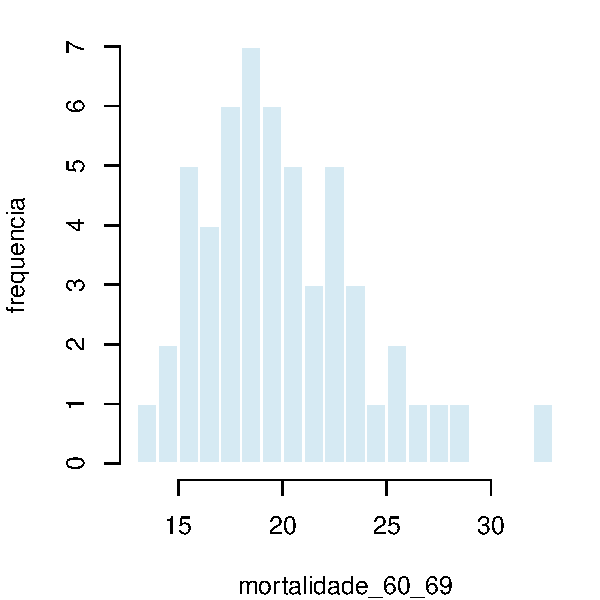
\includegraphics[width=0.52\linewidth]{figure/fig-resposta-1} 

}


\end{knitrout}
  \fonte{Elaborada pelos autores.}
\end{figure}

\textbf{Veredito.} A pergunta se sustenta. O modelo base atinge um RMSE de $3,84$, enquanto a inclusão dos preditores \texttt{municipio} e \texttt{ano} reduz o erro para um RMSE de $2,20$ em validação cruzada, removendo $42,6\%$ do erro da linha de base.

A pergunta é \textbf{provisória}: será revista depois da Aula 12, pois a aplicação de árvores, \emph{ensembles} e técnicas de regularização pode refinar a abordagem e permitir testar interações mais complexas.

\postextual
\bibliography{referencias}

\end{document}
